\chapter{Circuits Analogiques de Base}
Dans ce chapitre, nous verrons comment les éléments non linéaires sont utilisés dans les circuits électriques. Nous discuterons du concept d'une droite de charge, à la fois statique et dynamique, et étudierons la réponse en petit signal d'un élément non linéaire, ce qui nécessite essentiellement une linéarisation autour d'un point de fonctionnement. Enfin, nous fournirons des modèles en petit signal pour les diodes et les transistors à hautes et basses fréquences.

\section{Éléments non linéaires dans les circuits}
\label{sec:nonlin_circuits}
Dans cette section, nous verrons comment les éléments non linéaires tels que les diodes et les transistors sont utilisés dans les circuits électriques. En principe, l'ajout d'un élément non linéaire rend l'analyse du circuit beaucoup plus difficile que les circuits avec seulement des éléments linéaires (résistances, condensateurs, inductances, \ldots). En pratique cependant, nous nous appuierons sur une méthode de résolution graphique, qui simplifie l'analyse tout en restant rigoureuse.
\subsection{La Diode comme Élément de Circuit}
Utilisons une diode comme élément discret dans un circuit électronique, comme dans la figure ci-dessous.

\begin{wrapfigure}{r}{3.5cm}
	\centering
	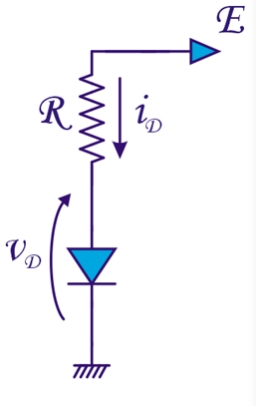
\includegraphics[width=3cm]{figures/ch02/diode1.jpg}
	\caption{}
	\label{fig:diode1}
\end{wrapfigure}
En appliquant la LKV, nous obtenons l'équation de la \textbf{droite de charge}:
$$
E - v_D = R \; i_D
$$
Cette équation doit être combinée avec la caractéristique I-V de la diode:
$$
i_D = \phi(v_D) = I_S (e^{v_D/v_{th}} - 1)
$$
D'un point de vue formel, nous avons deux inconnues, $v_D$ et $i_D$, et deux équations, donc en principe, nous pouvons résoudre pour les deux inconnues. Cependant, il n'y a pas de solution analytique à notre problème, nous préférons donc une méthode graphique.\
Dans la figure \ref{fig:diode2}, nous combinons $i_D = \phi(v_D)$ (la courbe rouge) avec l'expression de la droite de charge (la ligne verte).

\begin{figure}[h!]
	\centering
	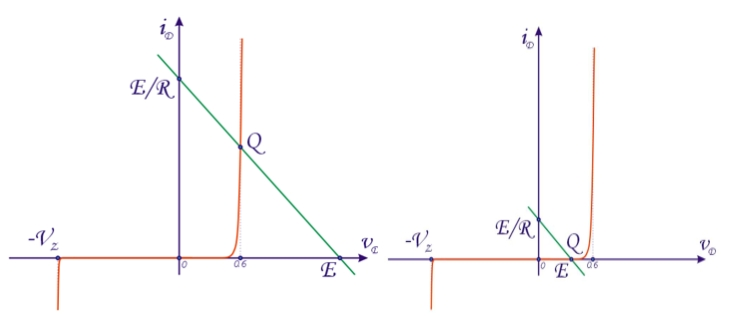
\includegraphics[width=12cm]{figures/ch02/diode2.jpg}
	\caption{I-V avec ligne de charge (a) avec $E > 0.6 V$ et (b) $E < 0.6$ V}
	\label{fig:diode2}
\end{figure}
Nous appliquons une simplification et supposons que $v_D = V_{DQ} \approx 0,6$ V. Le point de fonctionnement\footnote{La lettre $Q$ signifie \emph{quiescent}} $Q$ se situe à l'intersection des deux lignes. Pour que la diode conduise, nous pouvons immédiatement conclure, en comparant les deux figures, qu'il est nécessaire que $E > 0,6$ V $= V_{DQ}$. Le courant dans la diode est facilement calculé comme
$$
i_D \approx I_{DQ} = \frac{E - V_{DQ}}{R}
$$
Nous pouvons conclure que la diode conduira toujours tant que $E > 0,6$ V. Les variations de $E$ signifient seulement que la droite de charge se déplacera parallèlement. Le point de fonctionnement $(V_{DQ}, I_{DQ})$ ne peut se déplacer que verticalement en raison de la nature de $\phi(v_D)$ lorsque $v_D > 0,6$ V. Seulement lorsque $E$ devient inférieur à $0,6$ V la conduction s'arrête jusqu'à ce que nous atteignions la région Zener. Rappelons que le $0,6$ V est spécifique pour le silicium.\\

\begin{minipage}{.6\textwidth}
	Considérons par exemple le circuit de la figure \ref{fig:diode3}. Il n'est pas évident de savoir quand la diode va conduire, donc remplaçons la source de courant et la résistance par l'équivalent de Thévenin, à savoir une résistance $R_{th} = R$ et une source de tension $V_{th} = R I_0$ en \textbf{série} avec cette résistance. Ce circuit est identique à celui de la figure \ref{fig:diode1} avec une droite de charge passant par les points $(R;I_0, 0)$ et $(0, I_0)$. On peut conclure que la diode va conduire lorsque $V_{th} = R;I_0 > 0,6$ V. De plus, lorsque $R\rightarrow \infty$ et que la résistance devient un circuit ouvert, la droite de charge deviendra une ligne horizontale passant par $I_0$.
\end{minipage}
\begin{minipage}{.5\textwidth}
	\centering
	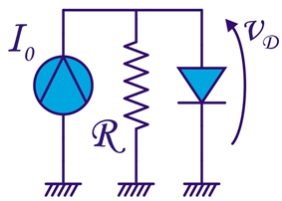
\includegraphics[width=5cm]{figures/ch02/diode3.jpg}
	\captionof{figure}{Avec source de courant}
	\label{fig:diode3}
\end{minipage}%

\subsection{Le BJT en tant qu'élément de circuit}
Un circuit typique à transistor bipolaire est représenté sur la figure \ref{fig:bjt_load1}(b). Pour analyser ce circuit, nous effectuons une coupure à l'entrée de la base et remplaçons la boucle de résistances $R_1$ et $R_2$ ainsi que la tension d'alimentation $E$ par le circuit équivalent de Thévenin, représenté sur la figure \ref{fig:bjt_load1}(a).

\begin{figure}[h!]
	\centering
	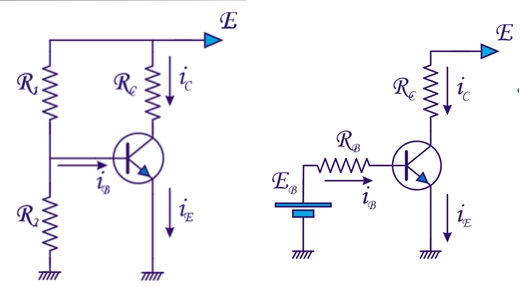
\includegraphics[width=12cm]{figures/ch02/bjt_load1.jpg}
	\caption{(a) Circuit à transistor et (b) simplifié avec Thévenin}
	\label{fig:bjt_load1}
\end{figure}

La tension de Thévenin $E_B$ et l'impédance $R_B$ peuvent être facilement calculées en observant que (a) la tension à la base est le résultat de l'application d'un diviseur de tension à la tension d'alimentation $E$, et (b) que lorsque nous mettons à la masse la tension $E$ (comme requis par les règles de Thévenin), $R_1$ et $R_2$ sont en parallèle :
\begin{equation}
	\begin{split}
		E_B &= \frac{R_2}{R_1 + R_2} E \\
		R_B &= R_1 || R_2 = \frac{R_1 R_2}{R_1 + R_2}
	\end{split}
\end{equation}
Dans cette boucle de gauche, nous pouvons écrire :
\begin{equation}
	\begin{split}
		E_B - v_{BE} &= R_B \; i_B \\
		%E - v_{CE} &= R_C \; i_C
	\end{split}
\end{equation}
Considérons la boucle de droite, qui est composée de la résistance $R_C$ et de la tension $v_{CE}$. Dans cette boucle, nous pouvons écrire :
\begin{equation}
	\begin{split}
		%E_B - v_{BE} &= R_B \; i_B \\
		E - v_{CE} &= R_C \; i_C
	\end{split}
\end{equation}
Supposons que tous les courants sont constants et que le transistor est polarisé dans son point de fonctionnement. Nous indiquons cela en ajoutant un $Q$ aux courants et tensions, tout comme pour la diode. Avec cette convention, nous pouvons réécrire ces équations pour obtenir :
\begin{equation}
	\begin{split}
		I_{BQ} &= \frac{E_B - V_{BEQ}}{R_B}\\
		V_{CEQ} &= E - R_C ; I_{CQ}
	\end{split}
\end{equation}
avec $V_{BEQ} \approx 0.6$ V car nous voulons polariser la jonction base-émetteur dans la région avant (conductive). À partir de l'analyse de la diode, nous savons que ce sera le cas lorsque $E_B > 0.6$ V. Nous connaissons également la relation entre $I_{BQ}$ et $I_{CQ}$ (en négligeant tout courant de fuite) :
\begin{equation}
	\begin{split}
		I_{CQ} &= \beta \; I_{BQ}
	\end{split}
\end{equation}
où $\beta$ est donné par le fabricant et est généralement très élevé, mais peut varier beaucoup d'un transistor à l'autre. Avec cette équation, nous avons suffisamment d'informations pour calculer tous les courants et tensions :
\begin{enumerate}
	\item Nous connaissons $R_B$ et $E_B$, et nous supposons que $V_{BEQ} = 0.6$ V, donc nous pouvons calculer $I_{BQ}$.
	\item Nous connaissons $\beta$, donc nous pouvons calculer $I_{CQ}$.
	\item Nous pouvons maintenant calculer $V_{CE}$.
\end{enumerate}
Tous ces calculs peuvent être représentés graphiquement ; voir la caractéristique (idéalisée) du BJT dans la figure \ref{fig:bjt_load2}.
\begin{figure}[h!]
	\centering
	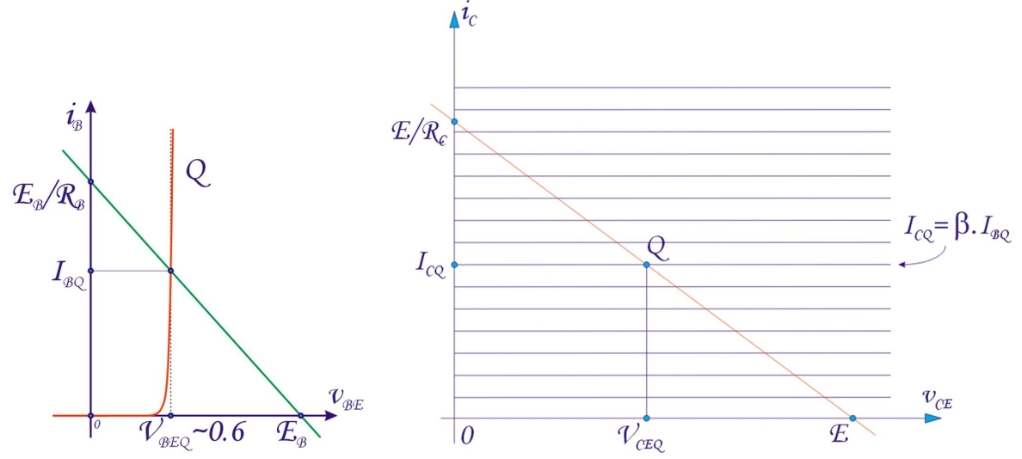
\includegraphics[width=12cm]{figures/ch02/bjt_load2.jpg}
	\caption{(a) Transistor circuit and (b) simplified with Thevenin} 
	\label{fig:bjt_load2}
\end{figure}
La figure de gauche représente la boucle de gauche, avec la droite de charge $E_B - v_{BE} = R_B ; i_B$ en vert et la caractéristique de la jonction $v_{BE}$ en rouge. L'intersection entre les deux fonctions est le point de fonctionnement $Q = (V_{BEQ}, I_{BQ})$. \
La boucle de droite est montrée dans le graphique de droite ; la ligne horizontale sur laquelle le transistor fonctionne est donnée par $I_{C} = \beta ; I_{B}$ et la droite de charge est donnée par $V_{CE} = E - R_C ; I_{C}$. Encore une fois, le point de fonctionnement est là où les deux lignes se croisent. \
Nous pouvons raisonner sur le fonctionnement du circuit en réfléchissant à ces figures. Par exemple, si $R_B$ diminuait, la pente de la droite de charge $I_B - V_{BE}$ augmenterait, de sorte que le point de fonctionnement $Q$ se déplacerait vers le haut et $I_{BQ}$ augmenterait. Cette augmentation provoquera une augmentation de $I_{CQ}$ dans le graphique de droite, et le point de fonctionnement se déplacera le long de la droite de charge vers un $I_C$ plus élevé et un $V_{CE}$ plus bas. \
Nous pouvons en conclure que :
\begin{itemize}
	\item La boucle de gauche détermine $I_{BQ}$.
	\item Par hypothèse, nous sommes dans le domaine de fonctionnement normal et $I_{CQ} = \beta I_{BQ}$.
	\item La boucle de droite donne $V_{CEQ}$.
	\item Étant donné $Q = (V_{CEQ}, ; I_{CQ})$, nous vérifions que nous sommes dans le domaine de fonctionnement normal.
\end{itemize}
Discutons maintenant de quelques cas limites :
\begin{itemize}
	\item Si $E_B < 0,6$ V, alors $V_{BEQ} < 0,6$ V. Alors $I_{BQ} \approx 0$ et $I_{CQ} \approx 0$ (en négligeant le courant de fuite). Voir la figure \ref{fig:bjt_load3}(a). Dans ce cas, le point de fonctionnement est $Q = (V_{CEQ} = E, 0)$ et le transistor est bloqué (\emph{mode de coupure}).
	\begin{figure}[h!]
		\centering
		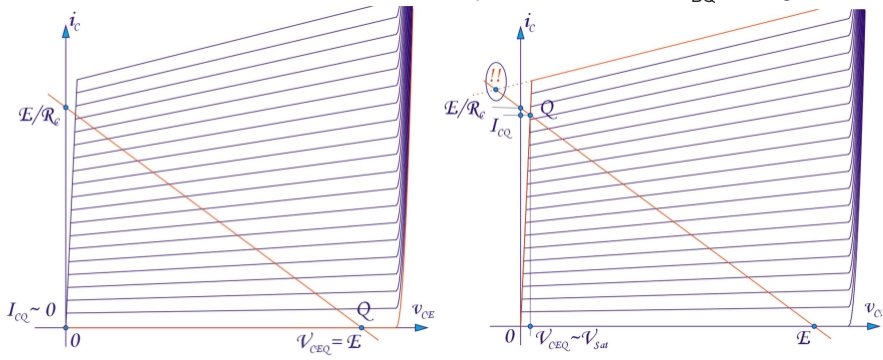
\includegraphics[width=14cm]{figures/ch02/bjt_load3.jpg}
		\caption{(a) $V_{BEQ} < 0.6$V et (b) $V_{CEQ} \approx V_{CE, Sat}$}
		\label{fig:bjt_load3}
	\end{figure}
	\item Au fur et à mesure que $V_{BEQ}$ et $I_{BQ}$ augmentent, $I_{CQ}$ deviendra plus grand et éventuellement $V_{CEQ}$ deviendra trop petit pour maintenir le transistor en mode actif. Ensuite, $I_{CQ} \ne \beta ;I_{BQ}$ et $V_{CEQ} \approx V_{CE, Sat}$. Dans ce cas, $I_{CQ} = \frac{E-V_{CE,Sat}}{R_C}$. Le transistor est \emph{saturé}.
\end{itemize}

\subsection{Le MOSFET en tant qu'élément de circuit}
Tout comme pour le BJT, nous considérons un circuit de polarisation pour le transistor MOSFET à canal n tel que présenté dans la figure \ref{fig:mos_load1}(a) et nous simplifions le circuit avec un circuit équivalent de Thévenin - comme nous l'avons fait auparavant - comme dans la figure \ref{fig:mos_load1}(b).
\begin{figure}[h!]
	\centering
	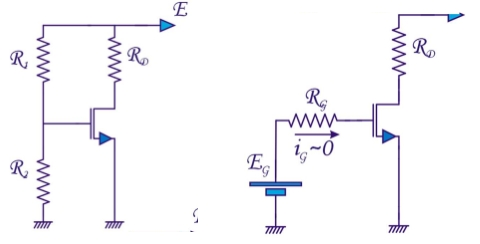
\includegraphics[width=10cm]{figures/ch02/mos_load1.jpg}
	\caption{(a) Circuit de transistor MOS et (b) simplifié avec Thévenin}
	\label{fig:mos_load1}
\end{figure}
avec
\begin{equation}
	\begin{split}
		E_B-G &= \frac{R_2}{R_1 + R_2} E \\
		R_G &= R_1 || R_2 = \frac{R_1 R_2}{R_1 + R_2}
	\end{split}
\end{equation}
Notez que le courant de la grille $I_G = 0$ car la grille est un condensateur où le courant continu est nul. Et tout comme pour le BJT, nous pouvons exprimer une équation pour la boucle gauche et droite :
\begin{equation}
	\begin{split}
		V_{GSQ} &= E_G \text{ car } I_{G} = 0\\
		I_{DSQ} &= \frac{\mu_n C_{ox}}{2} \frac{W}{L} (V_{GSQ} - V_T)^2 \text{ si } V_{GSQ} > V_T\\
		V_{DSQ} &= E - R_D ; I_{DSQ} \text{ si } V_{DSQ} > V_{GSQ} - V_T
	\end{split}
\end{equation}
La dernière condition est requise pour que le transistor soit saturé, ce qui est similaire au mode actif pour un BJT.\\
Nous pouvons également représenter ces équations graphiquement. La figure \ref{fig:mos_load2}(a) représente la relation quadratique entre $I_{DS}$ et $V_{GS}$ pour déterminer $V_{GSQ}$. Tant que $V_{DS} > V_{GSQ} - V_T$, la figure \ref{fig:mos_load2}(b) donne la valeur de $V_{DSQ}$.
\begin{figure}[h!]
	\centering
	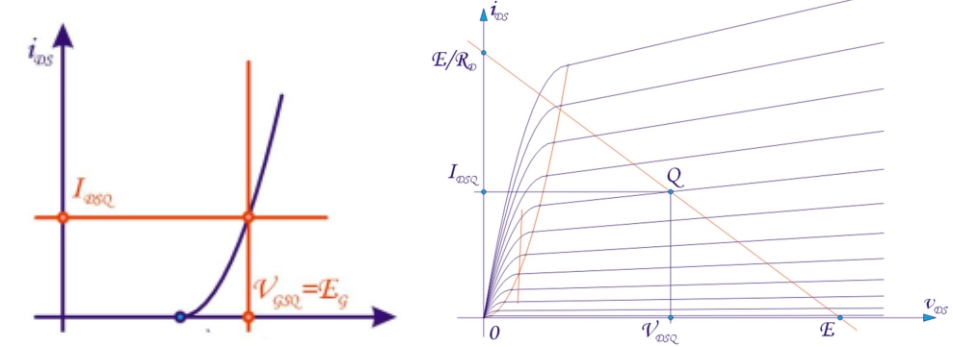
\includegraphics[width=14cm]{figures/ch02/mos_load2.jpg}
	\caption{(a) $i_{DS} = f(v_{DS})$ et (b) $I_{DS} = f(V_{DS})$}
	\label{fig:mos_load2}
\end{figure}


\subsection{Remarques supplémentaires}
Pour les deux types de transistors, il y a trois domaines de fonctionnement, comme indiqué dans la figure \ref{fig:transistor_overview}:
\begin{itemize}
	\item MOSFET : bloqué, saturé, linéaire
	\item BJT : bloqué, normal (ou actif), saturé
\end{itemize}
\begin{figure}[h!]
	\centering
	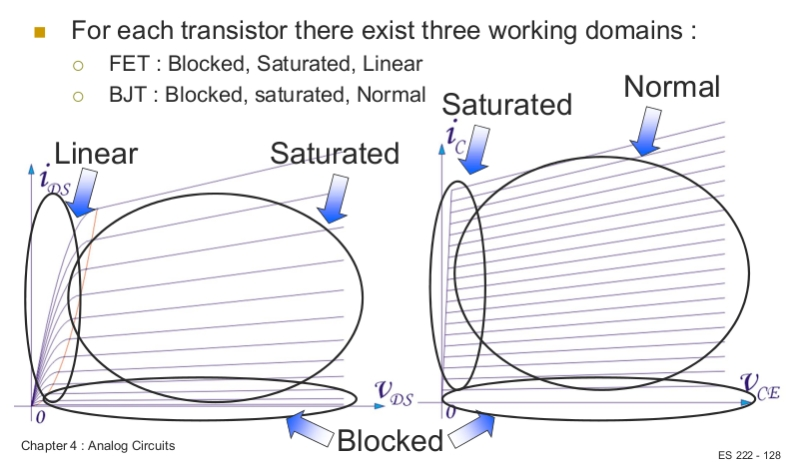
\includegraphics[width=12cm]{figures/ch02/overview.jpg}
	\caption{(a) $i_{DS} = f(v_{DS})$ et (b) $I_{DS} = f(V_{DS})$}
	\label{fig:transistor_overview}
\end{figure}
\subsection{Un circuit plus général}
\label{sec:general_circuit}
Pour améliorer la linéarité (voir le chapitre sur la rétroaction) et le polarisation du circuit, une résistance d'émetteur $R_E$ est souvent ajoutée, comme indiqué dans la figure \ref{fig:general1a}. Tout comme précédemment, le côté gauche est simplifié avec l'équivalent de Thévenin (voir \ref{fig:general1b}).

\begin{figure}[h!]
	\centering
	\begin{minipage}{.5\textwidth}
		\centering
		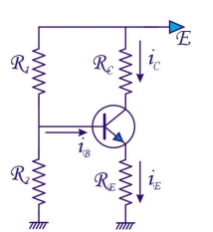
\includegraphics[width=4cm]{figures/ch02/general1a.jpg}
		\captionof{figure}{Circuit général}
		\label{fig:general1a}
	\end{minipage}%
	\begin{minipage}{.5\textwidth}
		\centering
		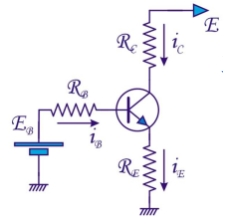
\includegraphics[width=5cm]{figures/ch02/general1b.jpg}
		\captionof{figure}{Simplification de Thévenin}
		\label{fig:general1b}
	\end{minipage}
	% \label{fig:explore}
\end{figure}
Encore une fois, nous pouvons écrire la LKC dans la boucle gauche et droite :
\begin{equation}
	\begin{split}
		E_B - V_{BEQ} &= R_B I_{BQ} + R_E I_{EQ} = R_B I_{BQ} + R_E (\beta + 1) I_{BQ} \\
		E_B - V_{BEQ} &= R_B \frac{I_{CQ}}{\beta} + R_E (\beta + 1) \frac{I_{CQ}}{\beta} \approx \frac{R_B}{\beta} I_{CQ} + R_E I_{EQ}
	\end{split}
\end{equation}
où nous avons utilisé $I_{CQ} = \beta I_{BQ}$ car nous supposons que nous travaillons dans la région de fonctionnement normal. Ces équations conduisent à des expressions pour le courant $I_{CQ}$ et la tension $V_{CEQ}$ :
\begin{equation}
	\begin{split}
		I_{CQ} &= \frac{E_B - V_{BEQ}}{\frac{R_B}{\beta} + R_E}\\
		V_{CEQ} &= E - (R_C + R_E) I_{CQ}
	\end{split}
	\label{eq:four_resitors1}
\end{equation}
Ils peuvent être tracés sur les différentes caractéristiques I-V comme sur la figure \ref{fig:general2}. Remarquez que la figure de gauche donne $i_C$ en fonction de $v_{BE}$. Puisque la relation entre $i_B$ et $v_{BE}$ est la caractéristique exponentielle de la diode, il en va de même pour la relation entre $i_C = \beta i_B$ et $v_{BE}$.

\begin{figure}[h!]
	\centering
	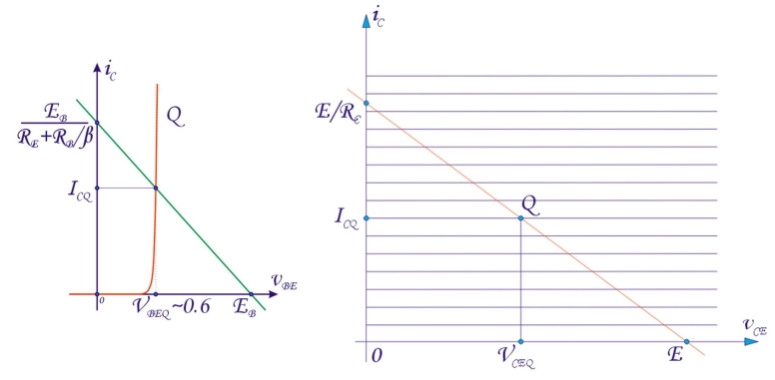
\includegraphics[width=12cm]{figures/ch02/general2.jpg}
	\caption{(a) Droite de charge : $I_{CQ} = \frac{E_B - V_{BEQ}}{\frac{R_B}{\beta} + R_E}$ (b) $V_{CEQ} = E - (R_C + R_E) I_{CQ}$}
	\label{fig:general2}
\end{figure}

On peut appliquer le même raisonnement au circuit MOSFET à $4$ résistances de la figure \ref{fig:mos_load3}, pour lequel nous pouvons également simplifier la boucle de gauche avec l'équivalent de Thévenin de la figure \ref{fig:mos_load4}.
\begin{figure}[h!]
	\centering
	\begin{minipage}{.5\textwidth}
		\centering
		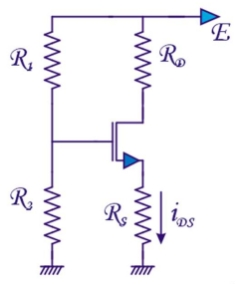
\includegraphics[width=5cm]{figures/ch02/mos_load3.jpg}
		\captionof{figure}{}
		\label{fig:mos_load3}
	\end{minipage}%
	\begin{minipage}{.5\textwidth}
		\centering
		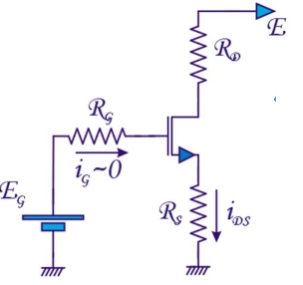
\includegraphics[width=6cm]{figures/ch02/mos_load4.jpg}
		\captionof{figure}{}
		\label{fig:mos_load4}
	\end{minipage}
	%	\label{fig:explore}
\end{figure}
Le point de fonctionnement $Q$ est déterminé par:
\begin{align*}
	&\text{L'équation de la boucle de gauche: } E_G - V_{GSQ} = R_S I_{DSQ} \
	&\text{La caractéristique du transistor: } I_{DSQ} = \frac{K}{2}\frac{W}{L} (V_{GSQ} - V_T)^2 \
	&\text{L'équation de la boucle de droite: } V_{DSQ} = E - (R_D + R_S)I_{DSQ}
\end{align*}
Pour trouver $V_{GSQ}$ et $I_{DSQ}$, utilisez les deux premières équations ; seule une racine est valide pour $V_{GSQ}$. $V_{DSQ}$ découle immédiatement de la troisième équation.
\section{Réponse en petit signal}
\label{sec:small_signal_response}
Dans cette section, nous allons introduire le concept de réponse en petit signal, c'est-à-dire comment les tensions et les courants dans un circuit changent lorsque nous appliquons une petite variation aux valeurs d'entrée. L'idée générale est que nous concevons le circuit de sorte qu'il fonctionne à un point de fonctionnement $Q$, et nous linéarisons le circuit autour de ce point de fonctionnement pour n'étudier que de petites déviations. Nous utiliserons la diode comme exemple. Dans la section \ref{sec:small_signal_model}, nous appliquons le même raisonnement aux transistors.\
Tout d'abord, nous introduisons une notation pour distinguer les quantités de grand signal des quantités de petit signal.

\begin{figure}[h!]
	\centering
	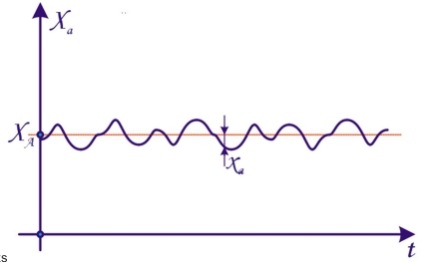
\includegraphics[width=8cm]{figures/ch02/small_signal_resp1.jpg}
	\caption{Signal quantities}
	\label{fig:small_signal_resp1}
\end{figure}
\begin{itemize}
	\item $x_A$: mesure d'une variable spécifique,
	\item $X_A$: la valeur moyenne de cette variable spécifique,
	\item $x_a$: variation de la variable spécifique autour de la moyenne $X_A$.
\end{itemize}
Consultez la figure \ref{fig:small_signal_resp1} pour une représentation visuelle de ces variables. Notez que seuls $x_A$ et $x_a$ varient dans le temps et que la valeur moyenne de $x_a$ est nulle : $\mathds{E}[x_a] = 0$.

\begin{minipage}{.6\textwidth}
	Appliquons cela au circuit diode simple. Dans la figure \ref{fig:small_signal_resp2}, l'alimentation comporte deux composantes : une tension fixe $E$, et une tension variable $e$ avec une valeur moyenne $\mathds{E}[e(t)] = 0$. Les quantités que nous recherchons, $v_D$ et $i_D$, peuvent être divisées en deux composantes : une valeur moyenne et une variation autour de cette moyenne.
	\begin{equation}
		\begin{split}
			v_D &= V_D + v_d\\
			i_D &= I_D + i_d
		\end{split}
	\end{equation}
\end{minipage}
\begin{minipage}{.4\textwidth}
	\centering
	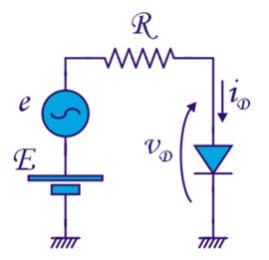
\includegraphics[width=5cm]{figures/ch02/small_signal_resp2.jpg}
	\captionof{figure}{}
	\label{fig:small_signal_resp2}
\end{minipage}

Supposons que $e=0$, c'est-à-dire que nous étudions le système sans variations. Si $E>0.6V$, nous pouvons écrire - comme nous l'avons fait précédemment - que :
\begin{equation}
	\begin{split}
		V_{DQ} &= 0.6V\\
		I_{DQ} &= \frac{E-V_{DQ}}{R}
	\end{split}
\end{equation}
Ainsi, nous déterminons le point de fonctionnement comme l'intersection entre la droite de charge et la caractéristique de la diode, comme dans la figure \ref{fig:small_signal_resp4}..

\begin{figure}[h!]
	\centering
	\begin{minipage}{.5\textwidth}
		\centering
		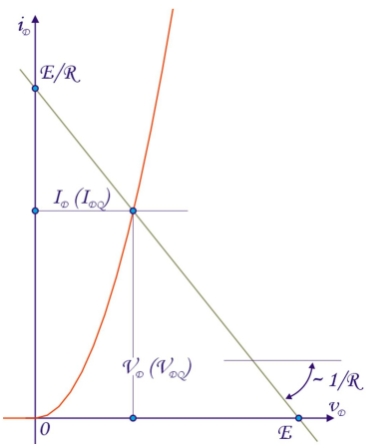
\includegraphics[width=6cm]{figures/ch02/small_signal_resp4.jpg}
		\captionof{figure}{Diode equation and load line}
		\label{fig:small_signal_resp4}
	\end{minipage}%
	\begin{minipage}{.5\textwidth}
		\centering
		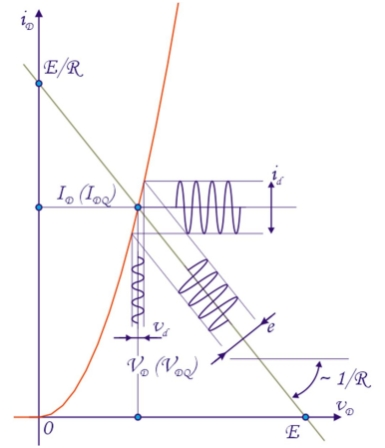
\includegraphics[width=6cm]{figures/ch02/small_signal_resp6.jpg}
		\captionof{figure}{Variations around $Q$}
		\label{fig:small_signal_resp6}
	\end{minipage}
	%	\label{fig:explore}
\end{figure}

Maintenant, supposons que $e\neq 0$. Cela modifie l'équation de la droite de charge :
\begin{equation}
	E+e - v_D = R;i_D
\end{equation}
Cette équation peut être réécrite comme :
$$
(E+e) - (V_{DQ} + v_d) = R (I_{DQ} + i_d)
$$
ou, puisque $E - V_{DQ} = R;I_{DQ}$ :
\begin{equation}
	e - v_d = R;i_d
\end{equation}
C'est l'équation de la droite de charge petit signal, où le centre du système de coordonnées est déplacé vers le point de fonctionnement $Q = (V_{DQ}, I_{DQ})$. La figure \ref{fig:small_signal_resp6} montre ce qui se passe : de petites variations de $e$ déplacent la droite de charge parallèlement à la droite de charge originale $E - V_{BEQ} = R;I_{DQ}$. Lorsque cette droite de charge en mouvement intersecte la caractéristique de la diode, de petites variations de tension $v_d$ et de courant $i_d$ apparaissent aux bornes de la diode. Nous pouvons déterminer la relation entre $v_d$ et $i_d$ :
\begin{equation}
	\begin{split}
		i_D &= \phi(v_D) \approx I_S e^{v_D/v_{th}}\\
		di_D &= \frac{I_S}{v_{th}} e^{v_D/v_{th}} dv_D \\
		\Rightarrow i_d &= \frac{i_D}{v_{th}} v_d
	\end{split}
\end{equation}
et finalement
\begin{equation}
	\begin{split}
		v_d = \rho_d;i_d \text{ avec } \rho_d = \frac{v_{th}}{I_{DQ}}
	\end{split}
\end{equation}
Nous avons effectivement linéarisé la caractéristique de la diode autour du point de fonctionnement. Localement, pour de petites variations, la diode fonctionne comme une résistance de valeur $\rho_d$.\
En faisant cela, nous avons transformé le problème original en deux sous-problèmes :
\begin{enumerate}
	\item Déterminer la solution en courant continu en résolvant (graphiquement) les équations à gauche de la figure \ref{fig:small_signal_resp7}. Cette solution détermine $Q$ et les paramètres de petit signal, tels que $\rho_d$.
	\item Résoudre un circuit linéaire où l'élément non linéaire a été remplacé par l'équivalent petit signal - une résistance dans le cas de notre diode. Voir la partie droite de la figure \ref{fig:small_signal_resp7}.
\end{enumerate}
\begin{figure}[h!]
	\centering
	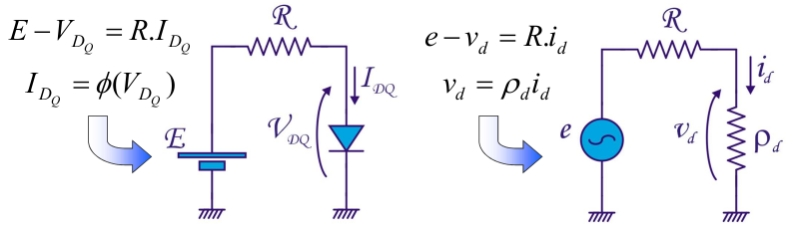
\includegraphics[width=12cm]{figures/ch02/small_signal_resp7.jpg}
	\caption{Quantités de signal}
	\label{fig:small_signal_resp7}
\end{figure}

Cependant, pour être exact, le modèle équivalent petit signal d'une diode n'est pas juste une résistance. Une jonction pn crée une région de charge d'espace sur son interface. Lorsque la tension aux bornes de la jonction change, des charges (à la fois $n$ et $p$) doivent être transportées vers et depuis la jonction pour augmenter ou diminuer le courant de saturation inverse. Cela signifie qu'une diode - ou toute jonction pn - est également capacitive. Ce phénomène de capacité de déplétion a déjà été expliqué dans la section \ref{sec:depletion_capacitance}.\
Pour modéliser ce comportement, nous remplaçons une diode dans un circuit équivalent petit signal par :
\begin{enumerate}
	\item Une résistance dynamique $\rho_d$, en parallèle avec
	\item Une capacité de jonction $C_j$, comme dans la figure \ref{fig:small_signal_resp8} (avec $\alpha = 1/2$). Cette capacité peut être négligée pour de faibles fréquences.
\end{enumerate}
\begin{figure}[h!]
	\centering
	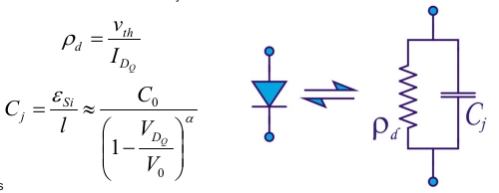
\includegraphics[width=10cm]{figures/ch02/small_signal_resp8.jpg}
	\caption{Modèle petit signal d'une diode}
	\label{fig:small_signal_resp8}
\end{figure}

Enfin, pour établir le circuit équivalent petit signal :
\begin{itemize}
	\item Nous remplaçons tous les dispositifs non linéaires par leur modèle petit signal (comme celui de la figure \ref{fig:small_signal_resp8} pour la diode).
	\item Nous remplaçons toutes les sources de tension indépendantes par un court-circuit (c'est-à-dire $E=0$) car nous supposons qu'elles ne varient pas dans le temps.
	\item Pour la même raison, nous remplaçons toutes les sources de courant indépendantes par un circuit ouvert (c'est-à-dire $I=0$).
\end{itemize}

\section{Static and Dynamic Load lines}
In section \ref{sec:nonlin_circuits}, we saw the concept of a load line. However, there is more to it than we've seen up to now. The reason is the fundamental difference between the operating point $Q$ and the small-signal response. The former is fundamentally a DC concept, because there are no time-varying quantities involved. The small-signal response at the other hand deals with AC signals: signals that vary in time and thus have a non-zero frequency. Let's thus study a circuit that contains frequency-dependent components like capacitors or inductors.\\
Consider the circuit in figure \ref{fig:loadline1}, where a load charge $R_L$ is connected to the original diode circuit through a capacitor $C$. To compute the operating point $Q$, we assume $e=0$. Since the are no variations, the capacitor $C$ is an open circuit and the circuit is reduced to the one in figure \ref{fig:loadline2}. This is the same circuit as before, so we conclude that $V_{DQ} = 0.6$ V and the load line is $E-V_{DQ} = R\; I_{DQ}$. The operating point allows us to compute the small-signal resistance $\rho_d$ of the diode.

%\begin{figure}
\begin{minipage}{.5\textwidth}
	\centering
	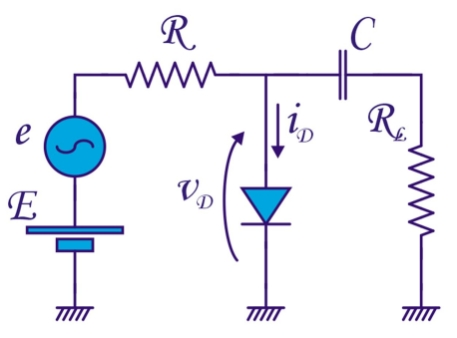
\includegraphics[width=6cm]{figures/ch02/loadline1.jpg}
	\captionof{figure}{Diode circuit with capacitor}
	\label{fig:loadline1}
\end{minipage}%
\begin{minipage}{.5\textwidth}
	\centering
	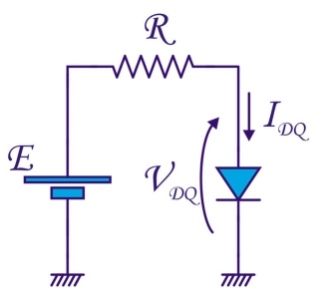
\includegraphics[width=5cm]{figures/ch02/loadline2.jpg}
	\captionof{figure}{Circuit to determine $Q$}
	\label{fig:loadline2}
\end{minipage}
%	\label{fig:explore}
%\end{figure}

For the small-signal response, we can't neglect $C$. We do replace the diode by a resistance $\rho_d$ (and neglect - for simplicity - the capacitance $C_j$) and obtain the circuit in figure \ref{fig:loadline3} with $E=0$. This circuit can be simplified with Thevenin's theorem, which gives the circuit in figure \ref{fig:loadline4} where we have made a cut just above $\rho_d$. $Z_{th}$ and $e_{th}$ can be computed as follows:
\begin{itemize}
	\item For $e_{th}$, we assume an open circuit, so no current through $\rho_d$. As such, we have a voltage divider consisting of resistors $R$ and $R_L$ and capacitor $C$. Let $Z_C$ be the series combination of $R_L$ and $C$, namely:
	\begin{equation}
		Z_C = R_L + \frac{1}{j\omega C} = \frac{1+j\omega R_L C}{j\omega C}
		\label{eq:Z_C}
	\end{equation}
	Then, we apply the expression for a voltage divider:
	\begin{equation}
		e_{th} = \frac{Z_C}{R+Z_C} e = \frac{\frac{1+j\omega R_L C}{j\omega C}}{R+\frac{1+j\omega R_L C}{j\omega C}} e = \frac{1 + j\omega R_L C}{1 + j \omega (R + R_L) C} e
	\end{equation}
	
	\item For $Z_{th}$, we replace $e$ by a short-circuit. $Z_{th}$ ts then the parallel combination of $R$ with $Z_C$:
	\begin{equation}
	Z_{th} = \frac{Z_C R}{Z_C + R} = R\;\frac{1 + j\omega R_L C}{1 + j \omega (R + R_L) C}
	\end{equation}
\end{itemize}
Obviously, the load line is different: at DC, it is $E - V_{DQ} = R \; I_{DQ}$, but at AC it is $e_{th} - v_d = i_d Z_{th}$. For high frequencies, we can simplify $Z_{th}|_{\omega \rightarrow \infty} = R\frac{R_L}{R+R_L}=R || R_L$  and the small-signal load line becomes $e_{th} - v_d = i_d (R || R_L)$ which has a different slope than the DC load line (keep in mind that the AC load line is centered at the operating point $Q$).

\begin{minipage}{.5\textwidth}
	\centering
	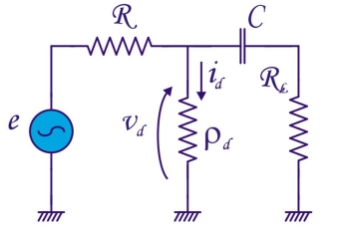
\includegraphics[width=8cm]{figures/ch02/loadline3.jpg}
	\captionof{figure}{Diode circuit with capacitor}
	\label{fig:loadline3}
\end{minipage}%
\begin{minipage}{.5\textwidth}
	\centering
	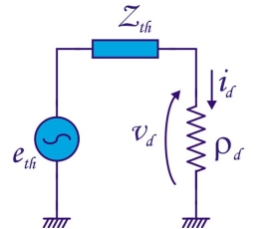
\includegraphics[width=6cm]{figures/ch02/loadline4.jpg}
	\captionof{figure}{Circuit to determine $Q$}
	\label{fig:loadline4}
\end{minipage}

Both load lines are show in figure \ref{fig:loadline5}, with in green the static load line (slope $=\frac{-1}{R_{stat}}$ where $R_{stat} = R$) and in blue the dynamic load line (slope $=\frac{-1}{R_{dyn}}$ where $R_{dyn} = R || R_L$).\\

\begin{figure}[h!]
	\centering
	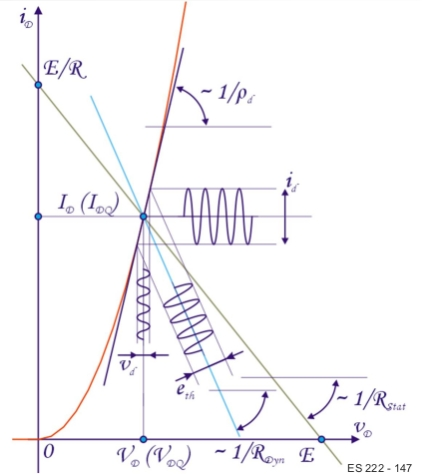
\includegraphics[width=8cm]{figures/ch02/loadline5.jpg}
	\caption{Static (green) and dynamic (blue) load lines}
	\label{fig:loadline5}
\end{figure}
We conclude that there are two load lines:
\begin{enumerate}
	\item The \emph{static} load line, determined at zero frequency (DC) and used to place the operating point.
	\item The \emph{dynamic} load line, at the frequency of interest, which typically is high enough so that we can simplify the impedance. It determines how the operating point will move (the small-signal response).
\end{enumerate}
The later remark implies that there is a critical frequency from which the capacitor $C$ can be neglected. From equation \ref{eq:Z_C}, we see that this impedance has a pole in $\omega=0$ and a zero in $\omega = 1/(R_L C)$. For pulsations higher than $\frac{1}{R_L C}$ , the impedance becomes frequency-independent and is equal\footnote{Convince yourself by sketching the Bode graph} to $R_L$. Thus the circuit reduces to the one in figure \ref{fig:loadline6}. It is this circuit that determines the dynamic load line.

\begin{figure}[h!]
	\centering
	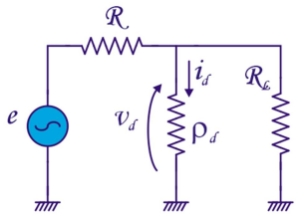
\includegraphics[width=6cm]{figures/ch02/loadline6.jpg}
	\caption{Circuit to determine the dynamic load line}
	\label{fig:loadline6}
\end{figure}

\subsection{Transistors and Dynamic Load Lines}
Consider the circuit in figure \ref{fig:loadline7}. This is the same circuit as we saw in figure \ref{fig:general1}, but with a capacitor $C_E$ in parallel with the emitter resistance $R_E$.
\begin{figure}[h!]
	\centering
	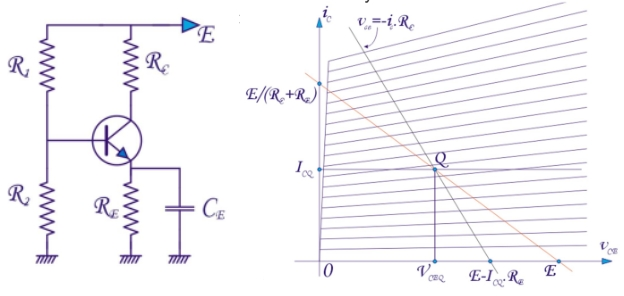
\includegraphics[width=14cm]{figures/ch02/loadline7.jpg}
	\caption{BJT circuit with emitter bypass capacitor $C_E$}
	\label{fig:loadline7}
\end{figure}
After simplifying the left part with the Thevenin theorem, we can establish the equation in the left loop, which hasn't changed from section \ref{sec:general_circuit}:
\begin{equation}
	E_B - V_{BEQ} = \bigg( \frac{R_B}{\beta} + R_E \bigg) I_{CQ}
\end{equation}
The equation in the right loop does change, with $Z_E = R_E || C_E = \frac{R_E}{1 + j\omega C_E R_E}$, and becomes
\begin{equation}
	v_{CE} = E - (R_C + Z_E)i_C
\end{equation}
which can be split into two equations:
\begin{enumerate}
	\item The DC operating point: 
		$$V_{CEQ} = E - (R_C + R_E)\; I_{CQ}$$,
	\item A small signal equation, valid for $\omega \gg \omega_0$:
		$$v_{ce} = -R_C \; i_c$$
\end{enumerate}
These static and dynamic load lines are represented in figure \ref{fig:loadline7} (red and green lines, respectively). The intersection of the dynamic load line with the horizontal axis is given by $E-R_E \; I_{CQ}$ because the voltage at the emitter is fixed (if $\omega$ is high enough) and equals $R_E \; I_{CQ}$. Hence, on the dynamic load line, the maximum swing of $v_{ce}$ is between $0$ and $E-R_E \; I_{CQ}$.
\section{Biasing}
In the previous section, we developed a way to determine the operating point of a transistor if the resistors are given:
\begin{itemize}
	\item Determine the current via the left loop: $E_B-V_{BEQ} = \bigg( \frac{R_B}{\beta} + R_E \bigg) I_{CQ}$ or $E_G - V_{GSQ} = R_S I_{DSQ}$.
	\item Determine $V_{CEQ}$ or $V_{DSQ}$ based on the right loop, and check wether we are in the normal (saturation) region of the transistor (i.e. $V_{CEQ} > 0.6$ V or $V_{DSQ} > V_{GSQ} - V_T$).
\end{itemize}
However, many values are not exactly known:
\begin{itemize}
	\item $V_{BEQ}$ varies over a specific production lot,
	\item $\beta$ depends on $i_C$, and varies (from -50\% to +200\%) over a specific lot,
	\item $V_T$ is only specified with a certain precision,
	\item $K = \mu_n C_{ox}$ (or $\mu_p C_{ox}$) is only specified with a certain precision,
	\item All these parameters vary with temperature.
\end{itemize}
This section will describe a method to choose the biasing resistors ($R_1$, $R_2$, $R_C$ or $R_D$ and $R_E$ or $R_S$) such that variation in the parameters above has minimal impact on the quiescent currents and voltages for which the circuit is designed.
\subsection{BJT Biasing}
\label{sec:bjt_biasing}
The goal of BJT biasing is to choose $R_1$, $R_2$ and $R_E$ to reduce the impact of variations on $V_{BEQ}$ and $\beta$. Furthermore, $R_C$ will be chosen such that the operating point $Q$ lies in the middle of the normal operating region.\\
Consider the general four-resistor BJT circuit in \ref{fig:general1}(b). We reproduce the Thevenin simplification here for convenience.\\
As a reminder, the Thevenin voltage $E_B$ and impedance $R_B$ are derived from the biasing resistors $R_1$ and $R_2$ and the supply voltage $E$: $E_B = \frac{R_2}{R_1+R_2}E$ and $R_{B} = R_1 || R_2$.

\begin{minipage}{.6\textwidth}
	From this circuit, we see that:
	$$
	E_B - V_{BEQ} = \bigg( \frac{R_B}{\beta} + R_E \bigg) I_{CQ}
	$$
	which means that:
	$$
	I_{CQ} = \frac{E_B - V_{BEQ}}{\frac{R_B}{\beta} + R_E}
	$$
	To make $I_{CQ}$ independent from $\beta$, we should choose 
	
	
	\begin{equation}
		R_B \ll \beta \; R_E
		\label{eq:RB_condition}
	\end{equation}
	such that:
	\begin{equation}
		I_{CQ} \approx \frac{E_B-V_{BEQ}}{R_E}
		\label{eq:ICQ}
	\end{equation}
\end{minipage}
\begin{minipage}{.4\textwidth}
	\centering
	%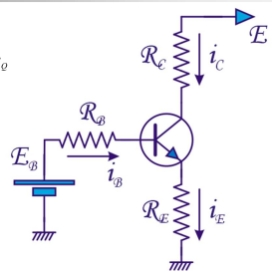
\includegraphics[width=6cm]{figures/ch02/biasing1.jpg}
	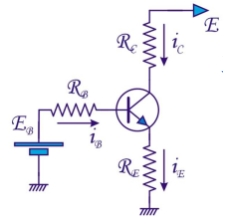
\includegraphics[width=5cm]{figures/ch02/general1b.jpg}
	\captionof{figure}{}
	\label{fig:biasing1}
\end{minipage}%

In this equation, we suppose that $E_B$ and $R_E$ are constant and can be produced with high accuracy (there is still a temperature dependence, but this is relatively low). Suppose that $V_{BEQ}$ can vary, which has an impact on $I_{CQ}$. This can be quantified with equation \ref{eq:ICQ}:
\begin{equation}
	\Delta I_{CQ} = \frac{\Delta V_{BEQ}}{R_E}
\end{equation}
A typical problem then goes as follows:
\begin{itemize}
	\item The limits of $V_{BEQ}$ are known, so we know $\Delta V_{BEQ}$
	\item The limits of $\beta$ are known: $(\beta_{min}, \beta_{max})$
	\item The value of $I_{CQ}$ is given, with a certain precision $\Delta I_{CQ}$
\end{itemize}
This problem can be solved by following these steps:
\begin{itemize}
	\item With $\Delta V_{BEQ}$ and $\Delta I_{CQ}$, determine $R_E = \frac{\Delta V_{BEQ}}{\Delta I_{CQ}}$,
	\item With $R_E$ and the equation of the left loop, determine $E_B=R_E \; I_{CQ} + V_{BEQ}$,
	\item With $\beta_{min}$, choose a $R_B$ such that $R_B \approx \beta_{min} R_E/10$. This guarantees that condition \ref{eq:RB_condition} is satisfied.
	\item With $R_B$ and $E_B$, determine $R_1$ and $R_2$ based on the Thevenin equations.
\end{itemize}
This procedure allows us to determine $R_1$, $R_2$ and $R_E$. The only remaining unknown is $R_C$. We will determine this resistor by requiring that the operating point $Q$ lies in the middle of the normal operating region. Refer to figure \ref{fig:loadline7} of the biasing circuit with bypass capacitor capacitor. We assume that $C_E \rightarrow \infty$, such that it is a short circuit for small signals\footnote{Or we assume that the only frequencies of interest are much higher that $ \omega_0/2\pi$.}. In this way, the static and dynamic load lines correspond to those of figure \ref{fig:loadline7}(b).\\
The slope of the dynamic load line is given by $R_C$. To determine this resistor, we need to set two points of the load line. We choose to limit the current $I_C$ between $0$ and $2 I_{CQ}$. This corresponds to a maximum attainable current swing. The minimum voltage is $V_{CE, Sat}$, because below this value the transistor goes into saturation. The maximum voltage is $E-R_E\;I_{CQ}$, as can be derived from the figure. Note that in AC, the emitter is grounded, so the voltage at the emitter is fixed. Hence we compute $R_E$ as the slope between these two points:
\begin{equation}
	R_C = \frac{E-R_E\;I_{CQ} - V_{CE,Sat}}{2 I_{CQ}}
	\label{eq:compute_RC}
\end{equation}
This reasoning is graphically represented in figure \ref{fig:biasing2}.
\begin{figure}[h!]
	\centering
	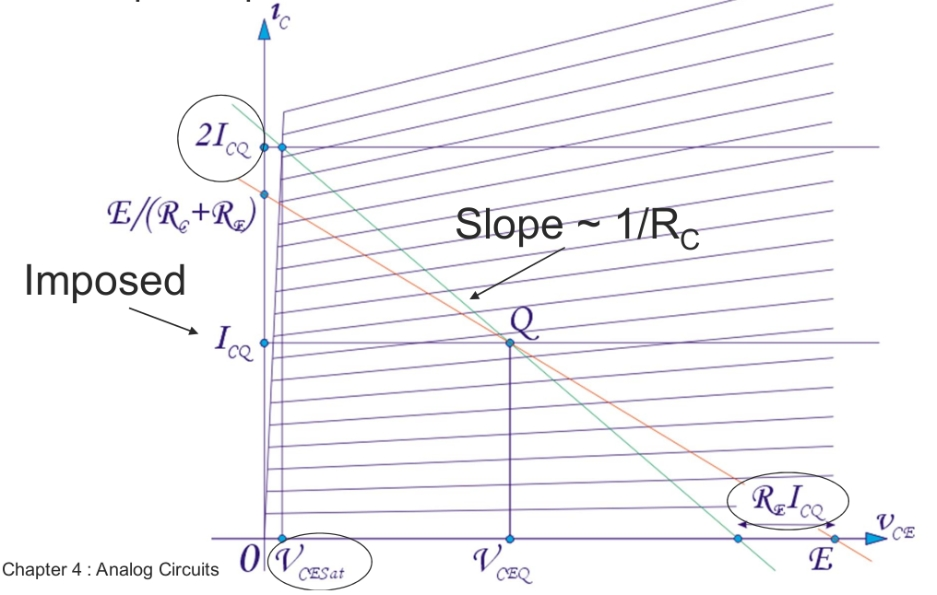
\includegraphics[width=10cm]{figures/ch02/biasing2.jpg}
	\caption{Determining $R_C$ to place in $Q$ in the middle of normal operating region }
	\label{fig:biasing2}
\end{figure}
\subsection{MOSFET Biasing}
\label{sec:mosfet_biasing}
The goal of MOSFET biasing is to choose $R_1$, $R_2$ and $R_S$ to reduce the impact of variations on $V_{T}$ and $K$. Furthermore, $R_D$ will be chosen such that the operating point $Q$ lies in the middle of the normal operating region.\\


\begin{minipage}{.5\textwidth}
	The circuit we consider is the one in figure \ref{fig:biasing3}. As always, we replace the maze on the left by the Thevenin equivalent with $E_G$ and $R_G$. We don't know the exact position of the $i_{DS}$ vs $v_{GS}$ curve because:
	\begin{itemize}
		\item The required value of $I_{DSQ}$ is only given within certain limits:\\ $I_{DSQ, min} < I_{DSQ} < I_{DSQ, max}$
		\item The manufacturer gives the value of $K=\mu C_{ox}$ within limits: $K_{min} < K < K_{max}$
		\item The same goes for the threshold voltage $V_T$: $V_{Tmin} < V_T < V_{Tmax}$.
	\end{itemize}
	
\end{minipage}%
\begin{minipage}{.4\textwidth}
	\centering
	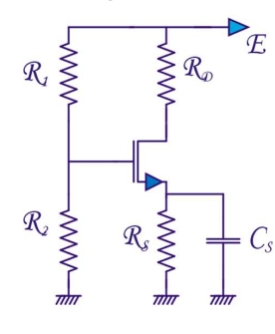
\includegraphics[width=5cm]{figures/ch02/biasing3.jpg}
	\captionof{figure}{}
	\label{fig:biasing3}
\end{minipage}


This allows us to draw a minimum (based on $V_{Tmax}$ and $K_{min}$) and maximum curve (based on $V_{Tmin}$ and $K_{max}$), as in figure \ref{fig:biasing4}. The intersection of these curves with resp. $I_{DSQ, min}$ and $I_{DSQ, max}$ gives two points on which the load line $E_G = v_{GS} + R_S i_{DS}$.  This is the only way to ensure that the intersection between load line and the real curve gives a current between $I_{DSQ, min}$ and $I_{DSQ, max}$. The slope of the line between these two points determines thus $R_S$, while the intersection with the $x$-axis sets $E_G$.\\
As there is no DC current through $R_G$, its value doesn't really matter for setting the operating point. We can choose $R_G$ freely and have an additional degree of freedom to determine $R_1$ and $R_2$ from the Thevenin equations\footnote{In the exercises, $R_G$ will be given.}.

\begin{figure}[h!]
\begin{minipage}{.5\textwidth}
	\centering
	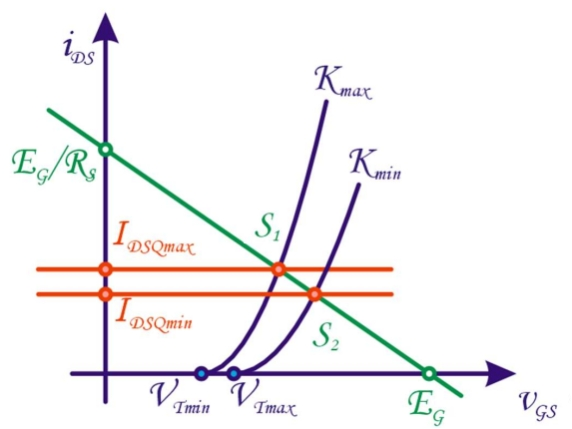
\includegraphics[width=\textwidth]{figures/ch02/biasing4.jpg}
	\captionof{figure}{}
	\label{fig:biasing4}
\end{minipage}%
\begin{minipage}{.5\textwidth}
	\centering
	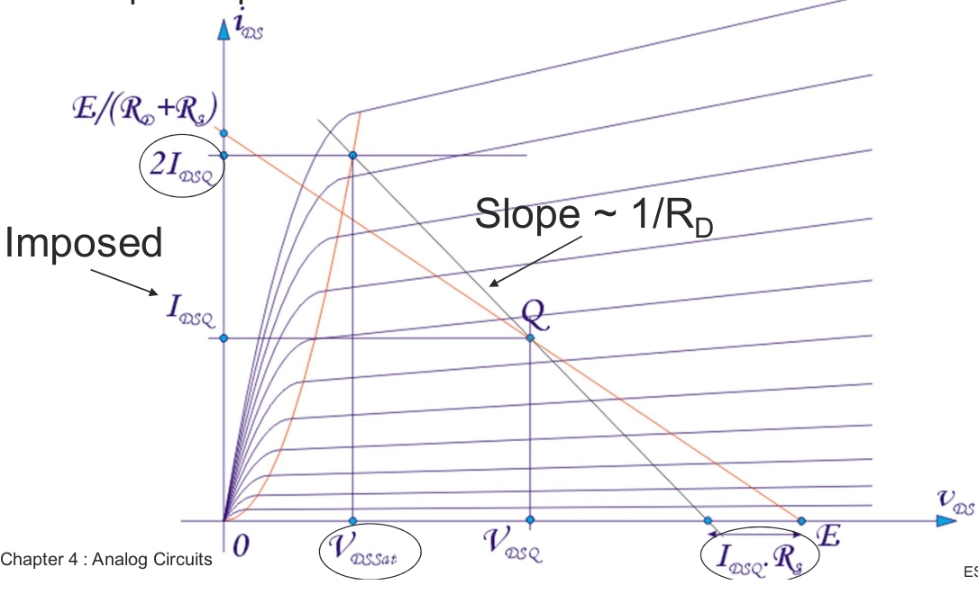
\includegraphics[width=\textwidth]{figures/ch02/biasing5.jpg}
	\captionof{figure}{}
	\label{fig:biasing5}
\end{minipage}
\end{figure}
To determine $R_D$, we apply the same reasoning as for the BJT: we want to place $Q$ in the middle of the saturation region. The minimum and maximum current is $0$ and $2\;I_{DSQ}$; the corresponding voltage range is $V_{DS,Sat} < V_{DS} < E - R_S\;I_{DSQ}$. The value of $V_{DS,Sat} = V_{GS} - V_T$, the minimum $V_{DS}$ to stay in saturation, has to be determined by solving $2 I_{DSQ} = \frac{K}{2} \frac{W}{L} V_{DS,Sat}^2$ because at the edge of saturation, the required current is $2 I_{DSQ}$:
$$
V_{DS,Sat} = \sqrt{\frac{2I_{DSQ}}{\frac{K}{2} \frac{W}{L}}}
$$
We then determine $R_D$ as:
\begin{equation}
	R_D = \frac{E - R_S\;I_{DSQ} - V_{DS,Sat}}{2\;I_{DSQ}}
\end{equation}
%\newpage
\section{The Small-Signal Model}
\label{sec:small_signal_model}
Basically, the small-signal model of a (non-linear) component is a representation of the component that can be used as a substitute when we consider small signals. It should only contain linear elements (resistors, inductors, capacitors, linearly depended current or voltage sources, \ldots) because it is obtained by linearizing the behavior of the component around an operating point $Q$.\\
In section \ref{sec:small_signal_response}, we established the small-signal model for the diode. This was a resistance $\rho_d$ in parallel with a capacitor $C_j$, as shown in figure \ref{fig:small_signal_resp8}. The values of both elements are set by the operating point $(V_{DQ},\; I_{DQ})$. In this section, we will develop the small-signal model for a bipolar junction transistor and for a MOSFET.

\subsection{BJT Small-Signal Model}
\label{sec:bjt_small_signal}
\begin{figure}[h!]
	\centering
	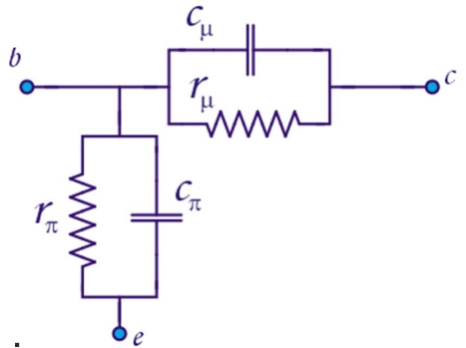
\includegraphics[width=0.4\textwidth]{figures/ch02/small_signal_model1.jpg}
	\caption{Just the pn-junctions}
	\label{fig:small_signal_model1}
\end{figure}
A bipolar junction transistor is nothing else than two pn-junctions put against each other. So we could just put the small-signal model of diode between base and emitter and between base and collector, as in figure \ref{fig:small_signal_model1} (for a npn transistor). 
However, in doing so, we don't have any component that mimics the transistor action, namely the dependence of $i_c$ on $i_b$. To do this, we define a current gain $h_{fe}$
\begin{equation}
	h_{fe} = \frac{di_C}{di_B} = \frac{i_c}{i_b} = \frac{d\beta i_b}{di_b} = \beta + \frac{d\beta}{di_b}i_b \approx \beta 
\end{equation}
and place a dependent current source $h_{fe} i_b$ between collector and emitter. Furthermore, since the output current between collector and emitter also depends on $v_{ce}$ because of the Early effect, we add an "Early" resistor $r_c$ between both terminals. Figure \ref{fig:small_signal_model2} gives the entire small-signal model for a npn BJT.
The different parameters depend on the biasing conditions:
\begin{itemize}
	\item Resistance $r_{\pi}$ is the diode resistance between base-emitter junction, thus: $r_{\pi} = \frac{v_{th}}{I_{BQ}}$.
	\item The base-collector junction is reversed biased, so $r_{\mu} \approx 0$.
	\item The Early resistance depends on the Early voltage $V_{E}$, which is about $40$V: $r_c \approx \frac{V_E}{I_{CQ}}$.
	\item Often, we express $i_c$ as function of $v_{be}$. The ratio between both is the \emph{transconductance} $g$:
	$$
	g = \frac{i_c}{v_{be}} = \frac{i_c}{r_{\pi} i_b} = \frac{h_{fe}}{r_{\pi}} \approx \frac{\beta I_{BQ}}{v_{th}} = \frac{I_{CQ}}{v_{th}}
	$$
\end{itemize}

By introducing this transconductance, we replace the current-dependent current source $h_{fe} \; i_b$ with a voltage-dependent current source $g \; v_{be}$. This is much better, because we can control $I_{CQ}$ by choosing $R_E$ and we can thus set $g$ with high precision. This is not the case for $\beta$, as explained previously. The result is shown in the model in figure \ref{fig:small_signal_model3}, which is also called \emph{Giacoletto's model}.

\begin{minipage}{.5\textwidth}
	\centering
	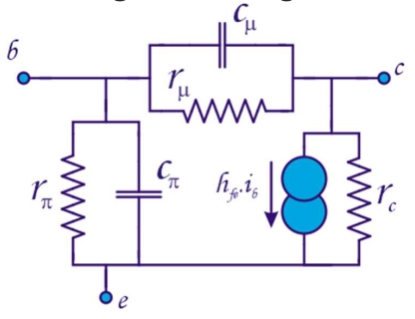
\includegraphics[width=7cm]{figures/ch02/small_signal_model2.jpg}
	\captionof{figure}{BJT small signal model}
	\label{fig:small_signal_model2}
\end{minipage}%
\begin{minipage}{.5\textwidth}
	\centering
	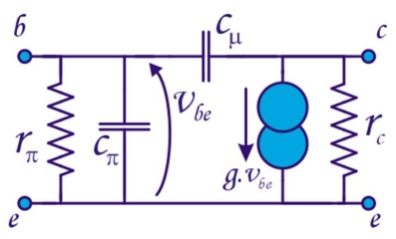
\includegraphics[width=7cm]{figures/ch02/small_signal_model3.jpg}
	\captionof{figure}{Giacoletto's model}
	\label{fig:small_signal_model3}
\end{minipage}

Note that $C_{\pi} \gg C_{\mu}$ because the width of the depletion zone is much smaller between emitter and base than between base and collector (the latter is reversed biased while the former is forward biased) and $C \sim \epsilon/t$ with $t$ the thickness of the depletion region. When working at low frequencies, the capacitors are omitted and replaced by open circuits to obtain the low-frequency model.


\subsection{MOSFET Small-Signal Model}
\label{sec:mosfet_small_signal}
For the MOSFET transistor, we observe that:
\begin{itemize}
	\item A voltage $v_{gs}$ causes a current between drain and source. We model this by a transconductance $g_m$.
	\item Because of channel-length modulation, $v_{ds}$ also has an impact on the current between drain and source. We model this with a resistor $r_{ds}$.
	\item The connections between gate and between source and gate and drain are capacitors: $C_{gs}$ and $C_{gd}$.
\end{itemize}

\begin{figure}[h!]
	\centering
	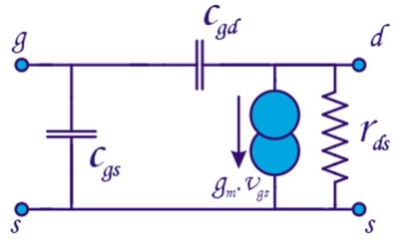
\includegraphics[width=7cm]{figures/ch02/small_signal_model4.jpg}
	\caption{MOSFET Small signal model}
	\label{fig:small_signal_model4}
\end{figure}

All these elements are represented in figure \ref{fig:small_signal_model4}. We can compute $g_m$, based on the $i_{DS} - v_{GS}$ characteristic (when $v_{GS} > V_T$):
\begin{equation}
	\begin{split}
		i_{DS} &= \frac{K}{2} \frac{W}{L}(v_{GS} - V_T)^2 \\
		\Rightarrow \frac{di_{DS}}{dv_{GS}} &= K \frac{W}{L}(v_{GS} - V_T)  = \frac{2i_{DS}}{v_{GS} - V_T}\\
		\Rightarrow g_m &= \frac{di_{DS}}{dv_{GS}}=\frac{i_{ds}}{v_{gs}} = \frac{2I_{DSQ}}{V_{DSQ} - V_T}
	\end{split}
\end{equation}
\\As for $r_{ds}$, this quantity is related to the channel-length modulation factor $\lambda$ from equation \ref{eq:sat_current2}:

\begin{equation}
	\begin{split}
		i_{DS} &= \frac{1}{2} \mu_n C_{ox} \frac{W}{L} (v_{GS} - V_T)^2 \; (1 + \lambda v_{DS})
	\end{split}
\end{equation}
This allows us to compute the change in $i_{DS}$ for small variations of $v_{DS}$:
\begin{equation}
	\begin{split}
		\frac{\partial i_{DS}}{\partial v_{DS}} &= \frac{1}{2} \mu_n C_{ox} \frac{W}{L} (v_{GS} - V_T)^2 \; \lambda \\
												&\approx \lambda \; I_{DSQ}
	\end{split}
\end{equation}
This expression is the conductivity $g_{ds}$ and thus $r_{ds} = \frac{1}{g_{ds}} \approx \frac{1}{\lambda \; I_{DSQ}}$.

\subsection{Orders of magnitude}
To estimate the values of the transistor parameters, we will assume that (a) a good value for the Early voltage $\approx 40$ V and that (b) the designer should choose a small $V_{DS,Sat}$ to maximize $g_m$, typically $\approx 200$ mV.\\
For the bipolar transistor, we observe that:
\begin{itemize}
	\item $g_{\pi} = \frac{1}{r_{\pi}}=\frac{I_{BQ}}{v_{th}} = \frac{I_{CQ}}{\beta v_{th}} = \frac{g}{\beta}$
	\item $g_c = \frac{1}{r_c} = \frac{I_{CQ}}{V_E} = \frac{v_{th}}{V_E} \frac{I_{CQ}}{v_{th}} \approx \frac{g}{1600}$
\end{itemize}
and thus: $g \gg g_{\pi} \gg g_c$.\\
For the MOSFET, we find that:
\begin{itemize}
	\item $g_{ds} = \frac{1}{r_{ds}}=\frac{I_{DSQ}}{V_E} = \frac{v_{DS, Sat}}{2 V_E} \frac{2I_{DSQ}}{v_{DS, Sat}} \approx \frac{g_m}{400}$
\end{itemize}
and thus: $g_m \gg g_{ds}$.
